\documentclass{standalone}
\usepackage{../../../../preamble_tikz}
\usepackage{../../../../preamble_math}


\begin{document}

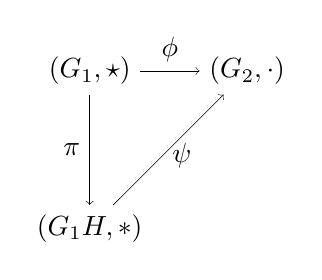
\begin{tikzpicture}
  %%% NODES
  \path (0,0) node(x) {$(G_1,\star)$}
  (2,0) node(y) {$(G_2,\cdot)$} (0,-2) node(z) {$\displaystyle\left(\quot{G_1}{H},*\right)$};
  %%% LINES
  \draw[very thin,->] (x) --node[above,midway] {$\phi$} (y);
  \draw[very thin,->] (z) --node[right,pos=0.45] {$\psi$} (y);
  \draw[very thin,->] (x) --node[left,midway] {$\pi$} (z);
\end{tikzpicture}

\end{document}